Magnetic field modified the particle momentum, in particular $p_{x}$ and $p_{y}$, changing the entrance position and incidence angle to the dRICH. In this section we look at the impact of this effect over the dRICH performance. Figure~\ref{fig:drich_p4_xy} show Cherenkov ring produce by 4~GeV electrons, pions, and kaons with and without magnetic field. 
\begin{figure}[h!tbp]
    \centering
    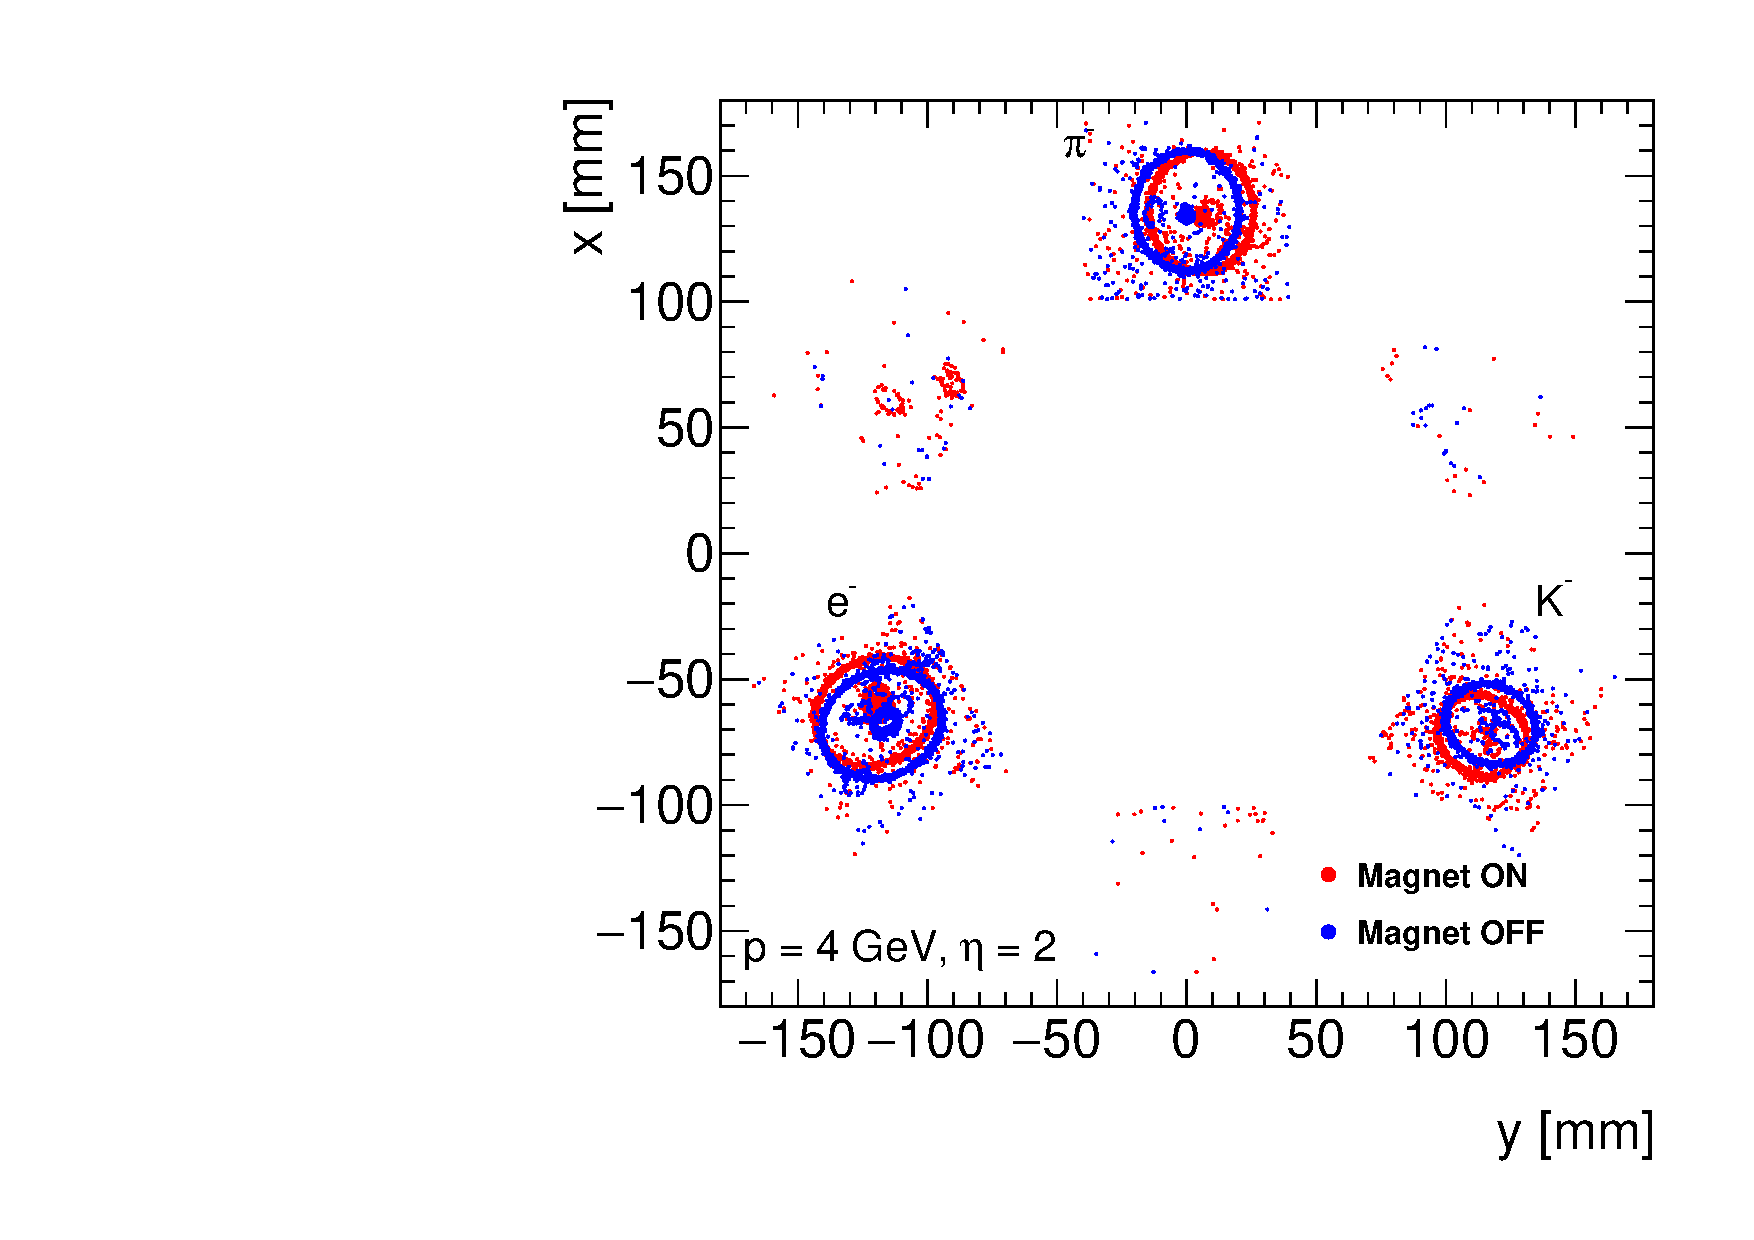
\includegraphics[width=0.5\textwidth]{figs/rings_xy_p4_fornote.pdf}
    \caption{dRICH hits, from events including 4~GeV electrons, pions, and kaons.}
    \label{fig:drich_p4_xy}
\end{figure}
To understand the impact of the magnetic field we look at the modification of the radius and width of the ring of electrons, pions, and kaons for three values of momentum, 1, 4, and 10~GeV. Figure~\ref{fig:drich_pX_e} shown dRICH hits centered at (0,0) in $(\eta,\phi)$ space with and without the magnetic field. We can see for 1~GeV electrons there is small smear of the inner (Gas) ring when the magnetic field is turned-on. 
\begin{figure}[h!tbp]
    \centering
    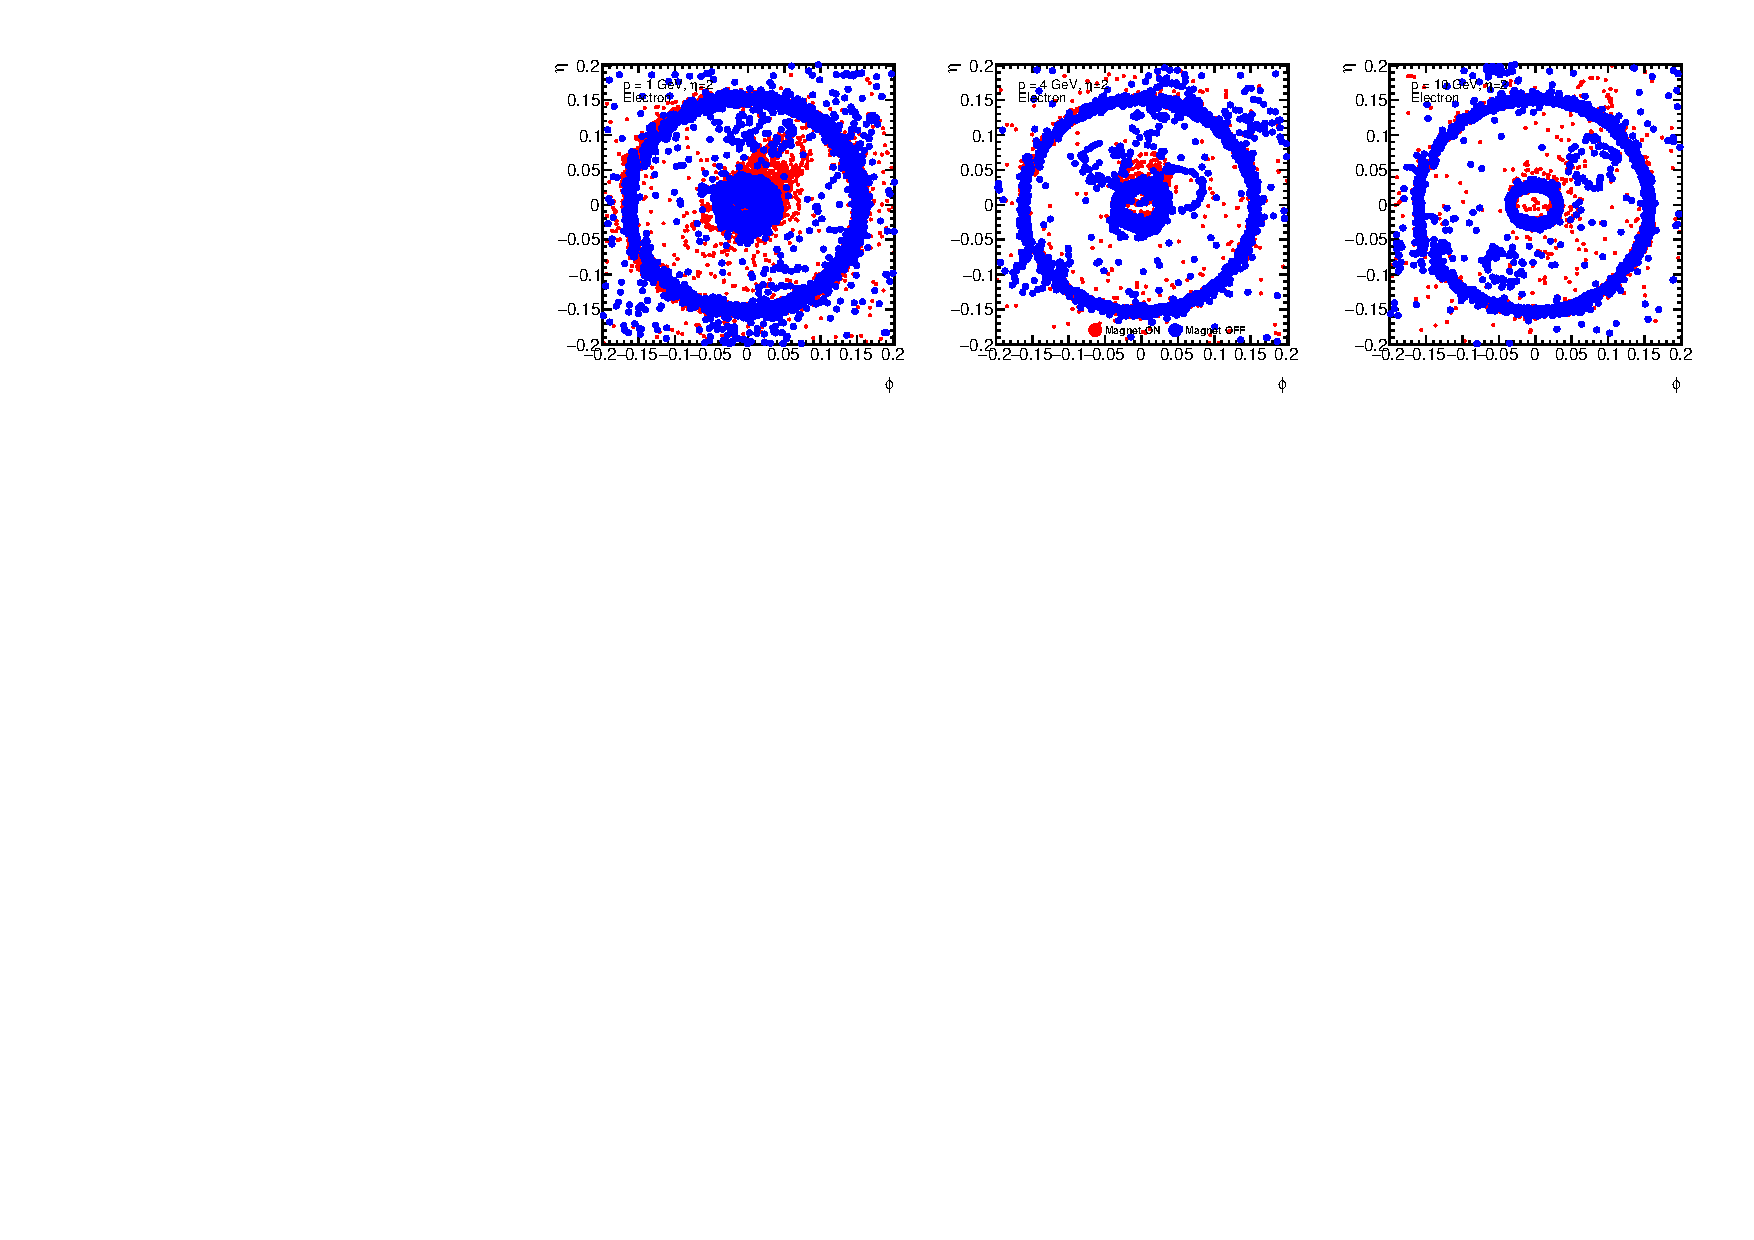
\includegraphics[width=0.9\textwidth]{figs/rings_etaphi_electron.pdf}
    \caption{dRICH hits for 1, 4 and 10~GeV electron events.}
    \label{fig:drich_pX_e}
\end{figure}
The radius distribution is calculated as $R=\sqrt{\phi^{2}+\eta^{2}}$ for each dRICH hit, we can compare this with magnetic field turned-on and off. In Figure~\ref{fig:drich_radius_p1_ePiK} we can see a small tail in the radius distribution for Gas ring of low p electrons. This small modification in the radius width is not expected to cause a degradation in the PID performance.
\begin{figure}[h!tbp]
    \centering
    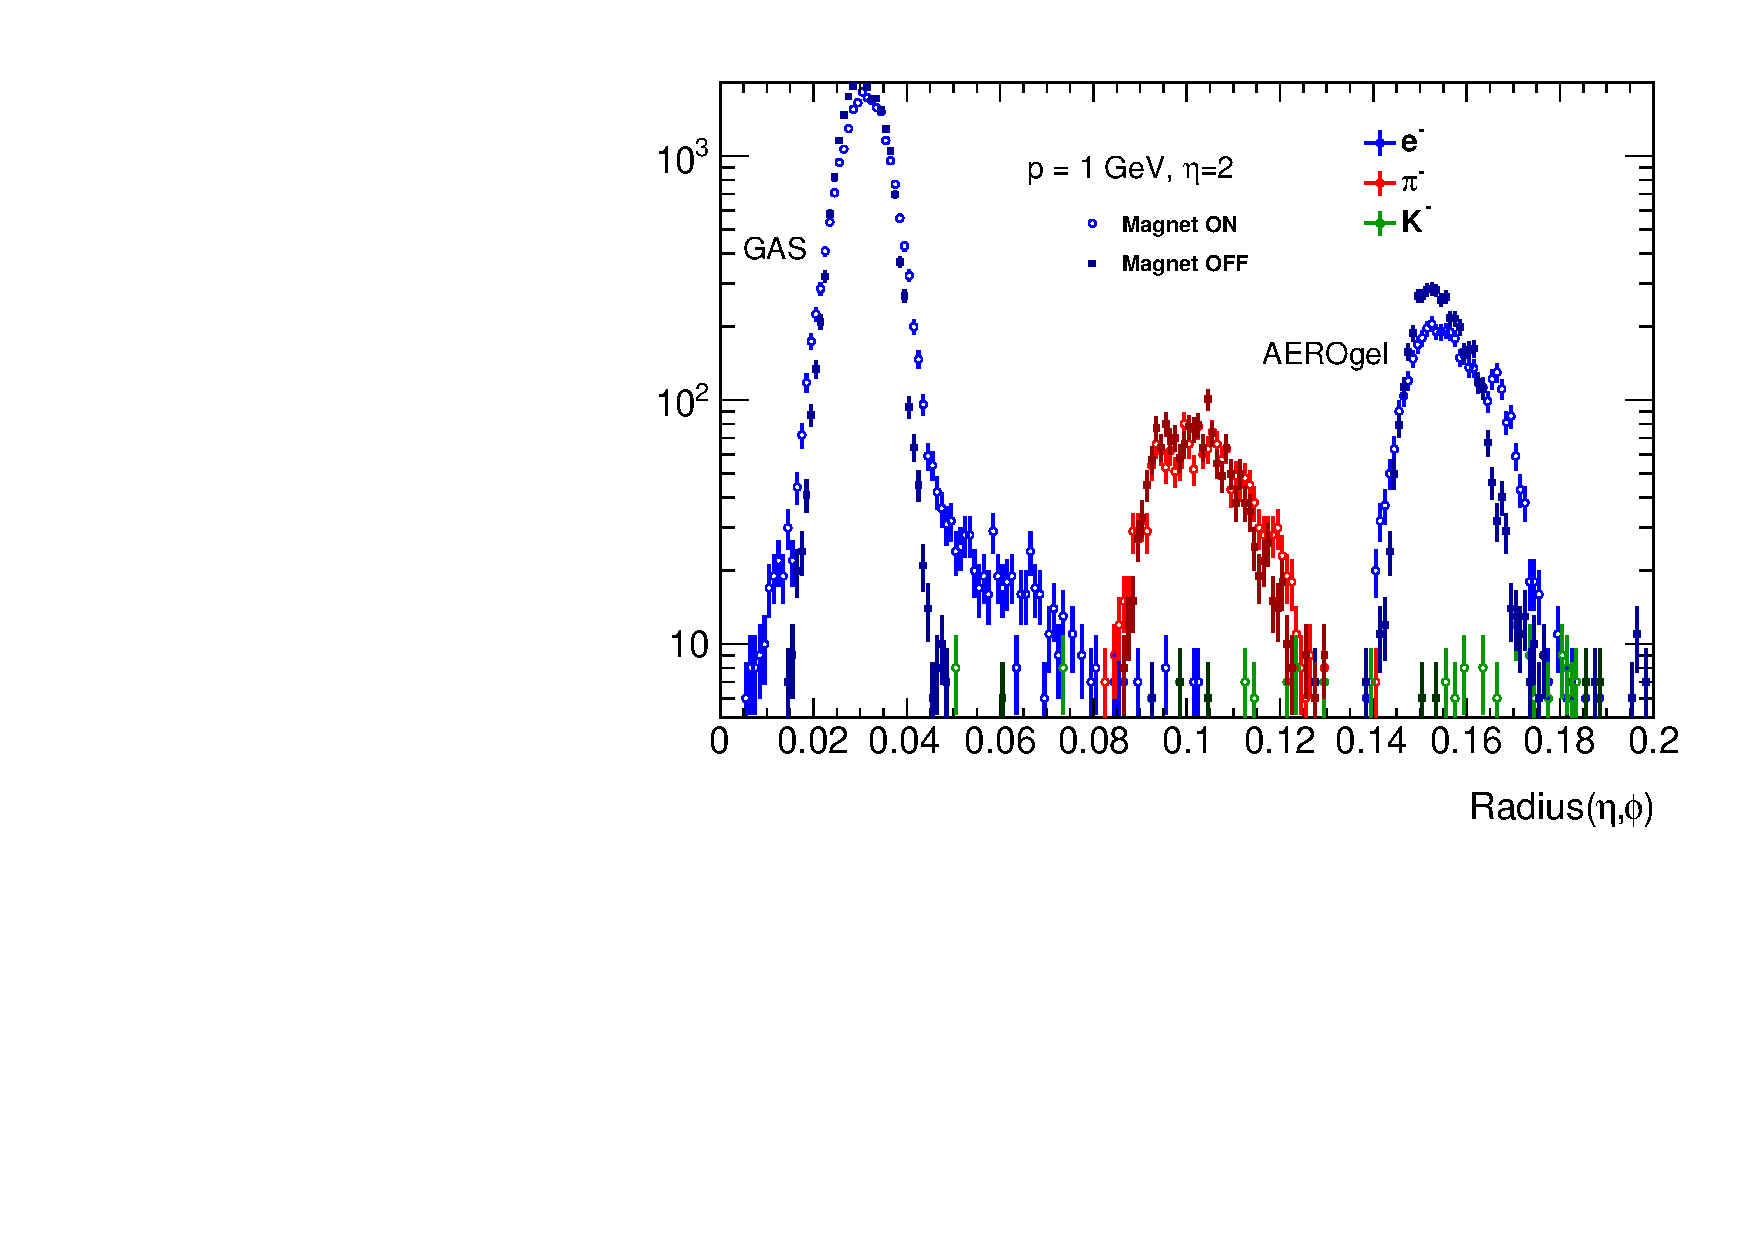
\includegraphics[width=0.7\textwidth]{figs/Radius_p1_shift.pdf}
    \caption{Radius distribution of 1~GeV electrons, pion and kaons.}
    \label{fig:drich_radius_p1_ePiK}
\end{figure}